\paragraph{Tolerance and scenario set.}
Table~\ref{tab:robust} varies the population tolerance $\varepsilon\in\{0.5\%,1\%,2\%\}$ (single scenario, $s=k-1$) and replaces the single 2020 presidential race by the minimum share over up to three statewide contests (presidential, and where available Senate and governor), for the six two-district states. Brackets are closed under Proposition~\ref{prop:mono} (a larger tolerance can only raise both ends; a larger scenario set can only lower them).

\begin{table}[!tbp]
\centering\small
\caption{Best-district ($q=1$) and second-best ($q=2$) share (\%) for tolerances 0.5\%, 1\% and 2\%, and for the robust scenario set at 1\% (number of contests in the last column). $s=k-1=1$.}\label{tab:robust}
\adjustbox{max width=\linewidth}{\begin{tabular}{llcccccc}
\toprule
State & Party & $q$ & $\varepsilon{=}0.5\%$ & $\varepsilon{=}1\%$ & $\varepsilon{=}2\%$ & robust $\Omega$, 1\% & contests \\
\midrule
New Hampshire & D & 1 & 57.01--57.5 & 57.02--57.5 & 57.14--57.5 & $<$50 & 3 \\
New Hampshire & D & 2 & 53.75--54.0 & 53.75--54.0 & 53.75--54.0 & $<$50 & 3 \\
New Hampshire & R & 1 & $<$50 & $<$50 & $<$50 & $<$50 & 3 \\
New Hampshire & R & 2 & $<$50 & $<$50 & $<$50 & $<$50 & 3 \\
Maine & D & 1 & 62.74--63.0 & 62.74--63.0 & 63.12--63.5 & 53.19--53.5 & 2 \\
Maine & D & 2 & 54.62--55.0 & 54.62--55.0 & 54.65--55.0 & $<$50 & 2 \\
Maine & R & 1 & 54.51--55.0 & 54.52--55.0 & 54.58--55.0 & 54.53--55.0 & 2 \\
Maine & R & 2 & $<$50 & $<$50 & $<$50 & $<$50 & 2 \\
Rhode Island & D & 1 & 70.12--70.5 & 70.12--70.5 & 70.52--71.0 & 70.31--70.5 & 2 \\
Rhode Island & D & 2 & 60.60--61.0 & 60.60--61.0 & 60.60--61.0 & 60.60--61.0 & 2 \\
Rhode Island & R & 1 & $<$50 & $<$50 & $<$50 & $<$50 & 2 \\
Rhode Island & R & 2 & $<$50 & $<$50 & $<$50 & $<$50 & 2 \\
Idaho & D & 1 & $<$50 & $<$50 & $<$50 & $<$50 & 2 \\
Idaho & D & 2 & $<$50 & $<$50 & $<$50 & $<$50 & 2 \\
Idaho & R & 1 & 75.52--76.0 & 75.52--76.0 & 75.62--76.5 & 74.53--75.5 & 2 \\
Idaho & R & 2 & 65.87--66.0 & 65.88--66.0 & 65.88--66.0 & 65.32--65.5 & 2 \\
West Virginia & D & 1 & $<$50 & $<$50 & $<$50 & $<$50 & 3 \\
West Virginia & D & 2 & $<$50 & $<$50 & $<$50 & $<$50 & 3 \\
West Virginia & R & 1 & 74.57--77.0 & 76.00--77.0 & 76.00--77.5 & 73.13--75.5 & 3 \\
West Virginia & R & 2 & 69.79--70.0 & 69.79--70.0 & 69.79--70.0 & 67.75--68.0 & 3 \\
\bottomrule
\end{tabular}
}
\end{table}

The tolerance matters little: doubling it from 1\% to 2\% shifts the certified bracket of the best district up by 0.4--0.5 point in Maine (Democrats) and Rhode Island (Democrats), where the two brackets are disjoint and the increase is therefore certified, by up to 0.1 point in New Hampshire, and by less than the bracket width elsewhere. Requiring the margin to hold in \emph{all} available contests matters a great deal for parties that did worse in the other races: New Hampshire Democrats, whose 57\% district relies on the presidential vote alone, can no longer make any district above 50\% in all of presidential, Senate and gubernatorial results (the 2020 governor's race was a Republican landslide); Maine Democrats fall from 62.7--63.0\% to 53.2--53.5\%; West Virginia Republicans from 76.0--77.0\% to 73.1--75.5\%; Montana Republicans from 67.5--69.5\% to 63.6--67.0\%. Rhode Island Democrats and Maine Republicans are unaffected. The seat--safety spectrum therefore doubles as a durability measure: the share cushion a district retains across elections is exactly its robust margin.

\begin{figure}[!tbp]
\centering
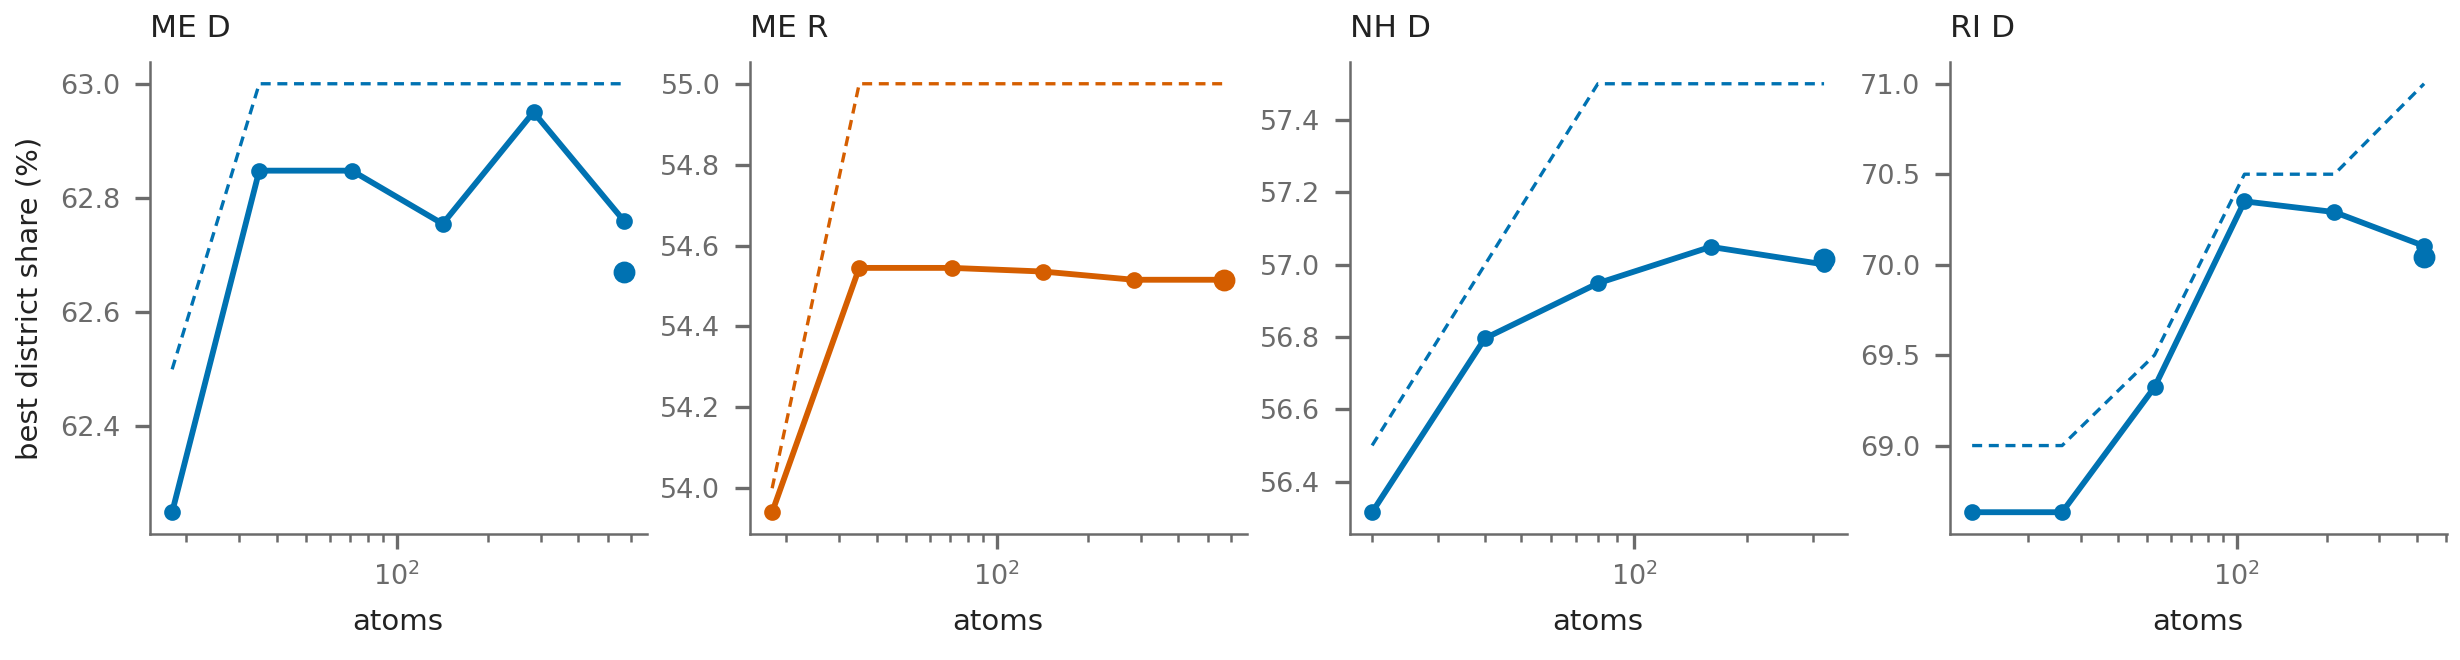
\includegraphics[width=\linewidth]{figs/ladder.png}
\caption{Resolution ladder: best-district share ($q=1$, $s=k-1$) when precincts are merged into fewer, larger atoms (plans keep merged atoms whole, so each rung is a lower-bound class for the next). Solid: best verified plan on the coarse instance; dashed: proven upper end for the coarse instance; large dot: the certified bracket at full precinct resolution. Non-monotone wiggles are heuristic search noise.}\label{fig:ladder}
\end{figure}

\paragraph{Resolution.}
Figure~\ref{fig:ladder} merges precincts, using the same homogeneity hierarchy as the algorithm, into $1/16,\dots,1/2$ as many atoms and recomputes the exact frontier. Because coarser atoms only shrink the plan class, each rung is a lower bound for the next, and the frontier saturates early: with a quarter of the precincts the best-district share is within 0.25 point of its precinct-level value in New Hampshire, Maine (both parties) and Rhode Island Democrats, and with a sixteenth it is within 0.7 point except in Rhode Island (1.5 points). This is evidence about sensitivity to \emph{coarser} atoms only; it does not bound what splitting precincts (or blocks, with an allocation model for the votes) could add.
